\section{Hj{\o}rring Library}
Hj{\o}rring Library aims to be distinguish itself from most other Danish libraries. This is seen by the fact that it is located inside a big shopping mall, and by their passion for being interactive. Among other things the library has its own cafeteria and bar where people can show up and eat their lunch, drink coffee or have a beer after work. The architecture also appears very modern; everything is in one big room, and there are many places for people to entertain themselves with other things than just traditional books. \\ Hj{\o}rring Library wants to be a place where people can "hang out" and relax, but also have fun or work. There are many unique pieces of furniture, creating a great environment for all purposes, and especially kids can have a fun time playing games (physical and digital) and record videos in the children zone.

Hj{\o}rring Library gets more than 1000 visitors every day, and the goal is to give them a new and exiting experience every time they visit. One way to achieve this is by having various themes that run throughout the whole library, changing every six weeks. These includes topics such as: Arabia, birds, fairy tales and "brown." The library will be decorated after these themes, so for example while the bird-theme was running all kinds of birds was exhibited around in the library, and bird songs was playing on speakers around the library.\\
These themes is an example of Hj{\o}rring Library eager to be experienced as the idea of serendipity, which basically describes a happy accident; something you didn't expect but turned out to be a pleasant surprise.

Hj{\o}rring Library is always looking for new projects that involves its visitors in new and engaging ways. Previously they have had Medialogy students come and do projects, and it turned out to be a success, so they are eager to try it out again. This is where our group comes into the picture. To us, this is a great opportunity to collaborate with a institution on a project in a "real-life" setting where people outside of the university will interact with our product.

In the period of this project Library Hj{\o}rring has chosen the topic of Christmas. This theme runs from the second week of November until the last week of December, 2012.

\subsection{Visitor data and placement of the canvas}
The library is divided into several parts, each aiming to give a different experience. As mentioned earlier it was important to the group that the placement of the canvas was in a central location. This would ensure that a lot of people would have the chance to interact with the program. In fact, the bookshelves we choose are just in the middle of the library, so it is almost impossible to not walk past it at some point (see figure \ref{fig:library_floorplans}).

\begin{figure}[htbp]
\centering
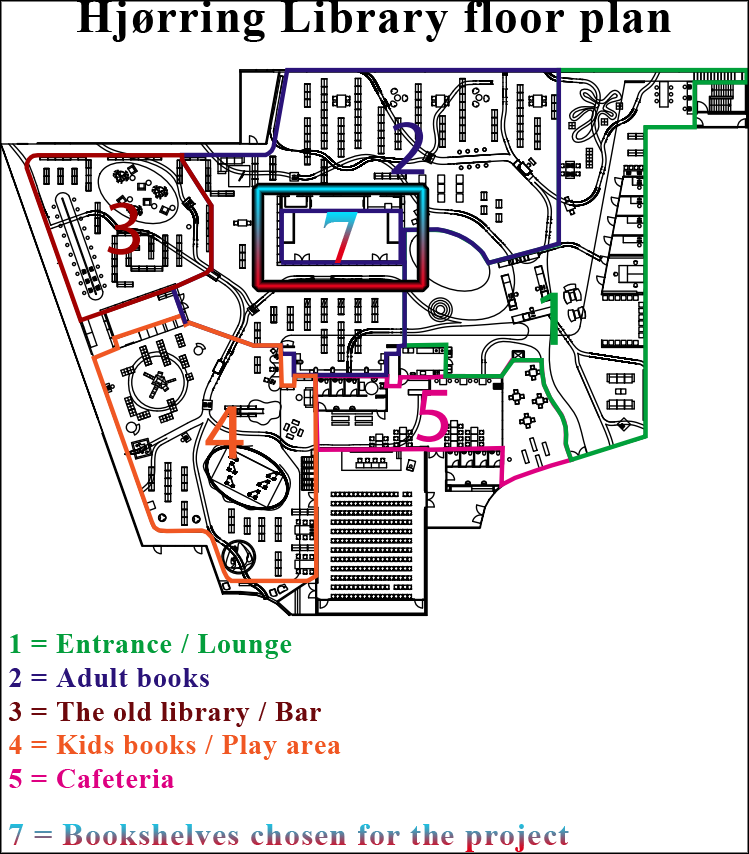
\includegraphics[width=0.80\textwidth]{Pictures/HjoerringLibrary/hjoerring_library_floorplans.png}
\caption{Hj{\o}rring Library is divided into multiple sections. We chose to use a big four-sided bookshelf in the core of the library. Image inspired by \citep{hjoerring_study}.}
\label{fig:library_floorplans}
\end{figure}

In 2010, \citep{hjoerring_study} did a survey to investigate people's habits and movement pattern at Hj{\o}rring Library. The found that an average visitor spends about half an hour at the library. Those in the age group between 0-10 years and 21-30 years spent most time, 34 and 44 minutes, while those between 41-50 and 61-70 years only spent 19 and 26 minutes during a visit.

Several cylinder and flow maps were made to visualize the gathered data, as shown in figures \ref{fig:library_cylindermap} and \ref{fig:library_flowmap}.

\begin{figure}[htbp] \centering
\begin{minipage}[b]{0.45\textwidth} \centering
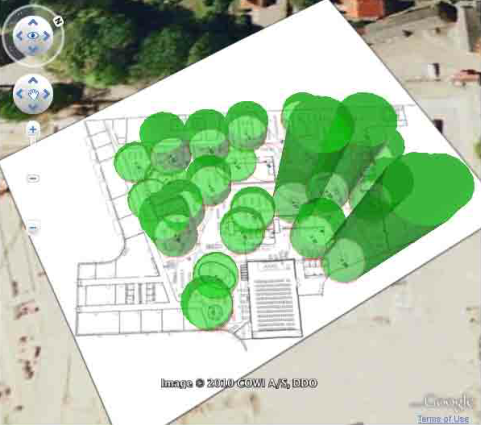
\includegraphics[width=1.00\textwidth]{Pictures/HjoerringLibrary/library_cylinder_diagram_24Nov.png} % Venstre billede
\end{minipage} \hfill
\begin{minipage}[b]{0.45\textwidth} \centering
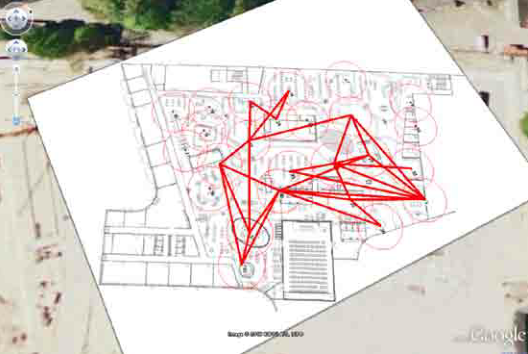
\includegraphics[width=1.00\textwidth]{Pictures/HjoerringLibrary/library_flow_Nov21.png} % Højre billede
\end{minipage} \\ % Captions og labels
\begin{minipage}[t]{0.45\textwidth}
\caption{Cylinder map showing accumulated visiting time at Hj{\o}rring Library Tuesday November 24 2010. Image created by \citep{hjoerring_study}.} % Venstre caption og label
\label{fig:library_cylindermap}
\end{minipage} \hfill
\begin{minipage}[t]{0.45\textwidth}
\caption{Flow map showing a visitor's movement between 10.20-11.15, Saturday November 21, 2010. Image created by \citep{hjoerring_study}.} % Højre caption og label
\label{fig:library_flowmap}
\end{minipage}
\end{figure}